\ifdefined\pdfminorversion\pdfminorversion=7\fi
\RequirePackage{xr-hyper}
\documentclass[manuscript]{acmart}

\usepackage{subcaption}
\usepackage{amsmath}
\usepackage{amsthm}
\usepackage{graphicx}
\usepackage{pdflscape}
\usepackage{booktabs}
\usepackage{longtable}
\usepackage{needspace}
\usepackage{array}
\usepackage{microtype}
\usepackage{placeins}
\usepackage{tikz}
\usepackage{pgfplots}
\usepgfplotslibrary{statistics}
\pgfplotsset{compat=1.17}
\usetikzlibrary{arrows.meta,positioning,fit,calc,shapes.geometric}
\usepackage[ruled,vlined,linesnumbered,longend]{algorithm2e}

\AtBeginDocument{%
  \providecommand\BibTeX{{Bib\TeX}}}
\acmJournal{TAAS}
\setcopyright{none}

\newtheorem{definition}{Definition}
\newtheorem{assumption}{Assumption}
\newtheorem{proposition}{Proposition}
\newtheorem{remark}{Remark}


\usepackage{afterpage}
\newcommand{\suppref}[1]{\ref{S-#1} of the Online Supplementary Material}
\newcommand{\mainref}[1]{\ref{M-#1} of the main paper}
\externaldocument[S-]{Online_Appendix}
\begin{document}

\title[Probe-Guided Rebalancing of Persistent Subscription Connections]{Probe-Guided Rebalancing of Persistent Subscription Connections with Greedy and Deep Q-Learning Control}

\author{Manish Kumar Agrawal}
\email{m\_agrawal@cs.iitr.ac.in}
\affiliation{%
  \department{Department of Computer Science and Engineering}
  \institution{Indian Institute of Technology Roorkee}
  \city{Roorkee}
  \state{Uttarakhand}
  \country{India}}

\author{Sandeep Kumar}
\email{sandeep.garg@cs.iitr.ac.in}
\affiliation{%
  \department{Department of Computer Science and Engineering}
  \institution{Indian Institute of Technology Roorkee}
  \city{Roorkee}
  \state{Uttarakhand}
  \country{India}}

\begin{abstract}
Transport load balancers cannot observe the application-level signals that
affect persistent subscription delivery. These include the subscriptions on
each connection, backlog per subscription, client acknowledgement capacity,
and pod reliability under subscription pressure. As a result, balanced
connection counts can still hide large differences in subscription counts and
queue backlog. We model client-side rebalancing as a sequence of decisions
based on partial observations. We present a probe-guided rebalancing framework
for persistent subscription transports, implemented and tested with STOMP. A
client combines telemetry from active persistent connections, local queue and
throughput counters, and one subscription-free connection that the existing
load balancer assigns to a random pod. The framework separates policy selection
from receipt-gated execution. It supports deterministic, pressure-aware greedy
control and Deep Q-Learning (DQL) over bounded actions. Both use subscription
count and backlog to assess a candidate; neither needs full cluster visibility.
The DQL policy additionally learns the tradeoff among backlog, imbalance,
throughput, and intervention cost. Execution guards block infeasible actions.
When migration is selected, the probe is promoted through a receipt-gated
standby, quiesce, drain, activate, detach, and old-socket retirement protocol.

In a locked scale-out simulator experiment, 20,000 subscriptions carry 775
million queued events on ten connections established on one Pod. Across 20
paired seeds, adding three Pods with unchanged connection placement yields
58,000 events/s. Probe-guided DQL and guarded-greedy migration yield 219,762
and 221,260 events/s, respectively. DQL reduces normalized backlog area by
12.30\% relative to unchanged placement (paired difference $-0.117504$;
95\% confidence interval $[-0.121210,-0.113345]$). The comparison establishes
the value of connection reassociation under the stated service model.
In a separate mixed-workload holdout, DQL improves mean composite reward by
0.0318 and reduces subscription-count variance by 90.0\% relative to the
two-dimensional heuristic, with a 4.5\% throughput tradeoff. Oracle Cloud
experiments establish execution of the mechanism: ten connection replacements
reassociate 4,000 of 20,000 subscriptions, and a loaded scale-out trial completes
three selective handoffs while retaining the other sessions and confirming
all 8,000 observed delivery ACKs. The framework therefore offers both a
transparent greedy policy and a learned multi-objective policy, with their
benefits evaluated separately from the shared handoff mechanism.
\end{abstract}

\begin{CCSXML}
<ccs2012>
 <concept>
  <concept_id>10010147.10010257.10010293.10010294</concept_id>
  <concept_desc>Computing methodologies~Reinforcement learning</concept_desc>
  <concept_significance>500</concept_significance>
 </concept>
 <concept>
  <concept_id>10010520.10010521.10010528</concept_id>
  <concept_desc>Computer systems organization~Cloud computing</concept_desc>
  <concept_significance>500</concept_significance>
 </concept>
 <concept>
  <concept_id>10011007.10010940.10010971.10010972</concept_id>
  <concept_desc>Software and its engineering~Message passing</concept_desc>
  <concept_significance>300</concept_significance>
 </concept>
 <concept>
  <concept_id>10011007.10010940.10010971.10010972.10010973</concept_id>
  <concept_desc>Software and its engineering~Publish-subscribe / event-based architectures</concept_desc>
  <concept_significance>300</concept_significance>
 </concept>
</ccs2012>
\end{CCSXML}
\ccsdesc[500]{Computing methodologies~Reinforcement learning}
\ccsdesc[500]{Computer systems organization~Cloud computing}
\ccsdesc[300]{Software and its engineering~Message passing}
\ccsdesc[300]{Software and its engineering~Publish-subscribe / event-based architectures}

\keywords{persistent connections, subscription rebalancing, deep Q-learning,
partial observability, probe promotion, greedy control, messaging systems, autonomic control}

\maketitle
\raggedbottom

\section{Introduction}

Distributed messaging systems support cloud-native and event-driven applications. Real-time analytics, notifications, workflow engines, and microservices need reliable event delivery as workloads change. Many deployments run several subscriber-service instances behind a transport-layer load balancer. Clients keep persistent STOMP/TCP, raw TCP, or WebSocket-style connections to these services.

Load balancing is therefore an important design concern. Poor distribution leaves some subscriber instances with growing backlogs and others with spare capacity. Clients then experience uneven delivery delays. Cloud resource-management reviews describe machine-learning methods for changing demand and capacity \cite{Khan2022MLCloudReview}. Deep-reinforcement-learning reviews also discuss adaptive policies for different resource types and competing objectives \cite{Zhou2024DRLCloudReview}. Conventional load balancers, however, usually distribute connections through policies such as round-robin or least-connections.

Those policies are simple and scalable, but connection count alone does not describe subscription-heavy messaging. A persistent connection may carry a few lightweight subscriptions or hundreds of high-rate subscriptions with growing queues. The load balancer may count both cases as one connection. The subscriber pod handles very different workloads in these cases. Its load depends on subscription count, backlog per subscription, and the client's message-processing and acknowledgement rates.

Subscriber-pod scale-out exposes this mismatch directly. If ten persistent
connections are established while only one pod exists, new pods increase
available processing capacity but do not change those established endpoints.
The client can use the new capacity by promoting a probe that reaches a
suitable pod and reassociating subscription-bearing connections to it. This
scale-out recovery is the central experiment in Section~\ref{sec:scaleout-recovery}.
The corresponding live handoff mechanism is examined during loaded Oracle
Cloud cluster scale-out in Section~\ref{sec:live-dql-scaleout}.

This mismatch creates two related problems. First, a client may reach a pod that already manages too many subscriptions, even when its connection count is acceptable. Second, the client may place too many subscriptions on one of its own connections. This can create local backlog even when the pod has enough capacity overall. A fixed connection pool cannot increase parallelism as subscription counts grow or event rates rise. Opening more connections without moving subscriptions, however, can leave the workload unevenly distributed.

Deep reinforcement learning has been used for hierarchical cloud scheduling \cite{Zhou2022DRLSelector}, multidimensional data-center allocation \cite{Wei2023TNSM}, and distributed cloud-edge offloading \cite{Nieto2024DRLOffloading}. Decentralized bandit methods select service instances from client QoS feedback \cite{Cilic2025} or coordinate edge offloading through server rewards \cite{Yahya2024}. BLOC also shows how client-side load balancing can use overload feedback without a central metadata store \cite{Bhattacharya2024}. These studies provide examples of adaptive control with limited information. Our focus is how the client changes persistent subscription connections. It retains a probed socket, promotes it only when the required checks pass, and transfers subscription ownership while preserving the durable queues.

Server placement, connection scaling, and subscription assignment depend on each other. Placement determines which pod a connection reaches. Scaling determines how many connections the client can use in parallel. Subscription assignment determines how evenly the work is spread across those connections. A practical controller must coordinate these decisions using only the information available to the client at runtime.

We propose an adaptive framework with coordinated control loops for persistent subscription messaging. It applies to long-lived STOMP/TCP, raw TCP, or WebSocket connections that carry multiple subscriptions and periodically report application-level statistics. The framework has three control loops at different system layers:

\begin{enumerate}
	\item A policy layer that chooses bounded actions from active-connection and probe statistics. We evaluate deterministic greedy rules and DQL as alternative selectors under partial observability.
	
	\item A client-side adaptive parallel connection scaling loop that adjusts the number of persistent transport connections based on total subscription count and per-subscription backlog characteristics.
	
	\item A connection-level load rebalancing loop that minimizes both subscription-count variance and per-subscription-backlog variance across scaled connections.
\end{enumerate}

Together, these loops let the client choose and carry out rebalancing actions without full cluster visibility. Both policy families use the client's own queues, active-connection statistics, and one retained probe assigned by the load balancer. The greedy policy responds to measured pressure and imbalance. DQL learns action values for the same operational objectives. The design keeps the existing transport load balancer.

\subsection*{Contributions}

The key contributions of this work are:

\begin{itemize}
	\item A client-side connection-replacement mechanism for persistent subscription transports. The client retains an authenticated, load-balancer-assigned probe and conditionally promotes that same socket, preserving the observed endpoint without requiring direct routing to a chosen Pod.
	
	\item A policy-independent separation of observation, action selection, and guarded execution. A pressure-aware greedy policy and a partially observable DQL policy use client-local queues and sampled Pod statistics. The experiments distinguish the benefit of the common mechanism from the choice of selector.
	
	\item Subscription- and backlog-aware connection scaling and two-dimensional connection rebalancing. These mechanisms distinguish adding transport parallelism, redistributing subscriptions across existing connections, and replacing a connection's delivery endpoint.
	
	\item An implemented receipt-gated handoff that retains subscription identity and durable queues. Standby target bindings, source quiescence, a fresh zero-in-flight check, target activation, and source retirement make migration an explicit protocol rather than an instantaneous reassignment.
	
	\item Complementary deployment and policy evidence: a 20,000-subscription Oracle Cloud cluster connection-replacement experiment, an isolated loaded scale-out trial with selective DQL handoffs, and controlled simulator comparisons and ablations. The evaluation separates executable handoff behavior, the benefit of rebalancing, and the contribution of learned action selection.
\end{itemize}

The contribution is not a new Q-learning update or a new greedy optimizer.
It is their integration with retained-probe selection and subscription-aware
connection replacement, supported by separate mechanism and policy tests.
Greedy control provides a transparent reference and a usable control policy;
DQL provides a learned choice among competing operational objectives. The
reported experiments evaluate them separately. They do not use a DQL model
to tune the scripted comparator or claim an evaluated hybrid policy.


\section{Background and Related Work}

\subsection{Persistent Messaging and Stream Processing}

We consider persistent subscription transports in which a client keeps a
long-lived connection to a subscriber service and multiplexes multiple
subscriptions over that connection. The abstraction covers STOMP-over-TCP,
custom TCP subscription streams, and WebSocket-based messaging. In each case,
the load created by one connection is not captured by the connection count
alone; it also depends on how many subscriptions are multiplexed over the
connection and how much backlog has accumulated behind those subscriptions.

Modern event-driven platforms and stream-processing engines face related
elasticity problems. Dynamic stream redirection can improve runtime elasticity
in distributed stream-processing systems \cite{Liu2020DrStream}. Cardellini
et al. survey runtime-adaptation strategies and organize them by their control
objectives and mechanisms \cite{Cardellini2022DSPAdaptation}. Recent adaptive
join-processing work also shows that workload redistribution can improve
latency and throughput under changing stream rates \cite{Sun2024AjStream}.
These studies motivate adaptive runtime control. Their actions change
operator placement, stream routing, or stateful processing inside the stream
runtime. They do not address the client-side persistent-transport problem in
which subscription count and per-subscription backlog must be balanced across a
client's own long-lived connections.

Fragkoulis et al. distinguish elasticity, reconfiguration, state management,
and fault tolerance in the evolution of stream-processing systems
\cite{Fragkoulis2024StreamEvolution}. This distinction matters here because
the durable queue stays in place: migration changes its subscription's delivery
owner, not the queue's stored contents. Transactional stream processing also
separates processing guarantees from ordinary stream execution
\cite{Zhang2024TransactionalStreams}. Accordingly, a completed connection
replacement is not, by itself, evidence of end-to-end exactly-once processing.

\subsection{Autonomic and Learning-Based Control}

Gheibi et al. organize machine-learning support for self-adaptation around
monitor--analyze--plan--execute feedback loops, including policy updates and
resource management \cite{Gheibi2021MLSelfAdaptation}. Our controller follows
that established pattern; DQL alone is not the differentiating mechanism.
The industrial survey by Weyns et al. also examines the practical motivations,
risks, and difficulties of deploying self-adaptation
\cite{Weyns2023Industry}. This motivates making the observation boundary and
the concrete connection-handoff procedure explicit.

Recent DRL literature is also clear about the risks of applying learning
methods directly to production systems. Partial observability, non-stationary
workloads, reward design, and safe online adaptation remain difficult
\cite{DulacArnold2021}. Cloud DRL surveys make the same point for operational
cloud control \cite{Zhou2024DRLCloudReview}. The closer load-balancing
comparisons already include decentralized operation. The QEdgeProxy preprint
describes multi-player bandits and per-client QoS feedback for selecting
service instances \cite{Cilic2025}. Yahya et al. combine mean-field bandits
with server-reward adjustment for decentralized task offloading
\cite{Yahya2024}. BLOC uses overload feedback and dynamic capacity estimation
without a centralized metadata store \cite{Bhattacharya2024}. Selvakumar
et al. use predicted waiting times and service-chain communication costs to
prioritize requests and select instances \cite{Selvakumar2023}. These
mechanisms provide direct comparisons for decision inputs and adaptive
selection. Our narrower distinction is conditional reuse of a retained probe
socket together with a concrete subscription-ownership handoff.

Negi et al. classify soft-computing approaches to VM- and physical-machine-level
load balancing \cite{Singh2023SoftCloudLB}. In our messaging setting, a bounded
action-template design limits the corresponding control space: the DQL agent
chooses among deployable rebalancing actions rather than directly searching
the full combinatorial subscription-assignment space.

Metzger et al. use feature models to guide exploration through large or
evolving adaptation spaces \cite{Metzger2024GuidedExploration}. Our bounded
templates reduce a different search space: the possible subscription moves
and connection replacements available to one client. Recent RS-DRL work
instead changes reward shaping during replay to manage uncertainty in
self-adaptation \cite{Kavianifar2026RSDRL}. We retain a conventional DQL
learner and specialize the observations, feasible actions, and handoff
semantics to persistent messaging.

\subsection{Research Gap and Novelty}

The comparison above identifies a specific gap in how actions are chosen and
carried out. Decentralized load balancing already exists. BLOC, QEdgeProxy, and
decentralized offloading already address decisions without a central
full-state controller. Our mechanism combines four requirements. It treats
pod subscription count and backlog as separate pressure signals. It tracks
the client's subscription-to-connection assignments. It promotes the same
authenticated probe socket only after checking that candidate. Finally, it
uses receipt-gated delivery handoff while durable queues stay in place.
These requirements
define the comparison in Table~\ref{tab:comparison_related_work}.

The proposed mechanism connects these concerns through an endpoint-preserving
probe workflow. The load balancer selects a reachable Pod when the probe is
opened; the selected policy then evaluates whether to use that already-established connection.
Promotion is conditional, not an automatic consequence of probing. An
admissible migration reuses the observed socket and transfers subscription
delivery ownership under the handoff contract, while the durable queues remain
stationary. This differs from choosing a Pod by name and opening another
load-balanced socket, whose endpoint could differ from the one evaluated.
Local subscription and backlog measurements also support scaling and
redistribution across existing connections. The contribution is this
partially observable control and execution mechanism, evaluated with established
greedy and Q-learning methods. Their comparison is specific to the measured workloads.
Table~\ref{tab:comparison_related_work} summarizes the
positioning of the proposed approach relative to representative literature.

\begin{table*}[t]
	\small
	\caption{Comparison of Representative Work and the Proposed Framework}
	\label{tab:comparison_related_work}
	\centering
	\setlength{\tabcolsep}{3pt}
	\renewcommand{\arraystretch}{1.08}
	\begin{tabular}{>{\raggedright\arraybackslash}p{0.17\textwidth}>{\raggedright\arraybackslash}p{0.18\textwidth}>{\raggedright\arraybackslash}p{0.17\textwidth}>{\raggedright\arraybackslash}p{0.18\textwidth}>{\raggedright\arraybackslash}p{0.18\textwidth}}
		\toprule
		\textbf{Work} & \textbf{Main focus} & \textbf{Observed information} & \textbf{Controlled object} & \textbf{How this work differs}\\
		\midrule
		BLOC \cite{Bhattacharya2024} & Request balancing and overload control & Overload feedback; no central metadata store & Request admission and server selection & Adds retained-socket promotion and subscription ownership transfer\\
		QEdgeProxy \cite{Cilic2025} & QoS-aware service selection & Client QoS outcomes; decentralized bandits & Service-instance selection & Preserves the probed endpoint during connection replacement\\
		Adaptive load balancing \cite{Selvakumar2023} & Service-chain latency & Predicted waiting times; inter-service costs & Request priorities and instance selection & Reassociates existing subscription-bearing connections\\
		Decentralized offloading \cite{Yahya2024} & Task distribution among edge servers & Unknown network information; adjusted server rewards & Offloading population control & Reassociates persistent subscription groups\\
		Per-device DRL \cite{Nieto2024DRLOffloading} & Energy- and latency-aware offloading & Device, server, channel, and task state & Local, MEC, or cloud task execution & Uses subscription counts and queued-event pressure\\
		Partial-observation DRL \cite{Hou2023PODRL} & QoE-aware distributed offloading & Partial observations; device QoE preferences & IoT task-offloading decisions & Evaluates a retained probe and transfers subscriptions\\
		Dr-Stream \cite{Liu2020DrStream} & Stream redirection and operator elasticity & Stream-runtime measurements & Operator instances and stream state & Keeps durable queues stationary during transport handoff\\
		Aj-Stream \cite{Sun2024AjStream} & Skew-aware stream joining & Predicted key frequencies; instance load & Key grouping and operator scaling & Moves subscription ownership while queues stay in place\\
		RL autoscaling \cite{AbdelKhaleq2021Autoscaling} & Microservice scaling thresholds & Resource demand and response-time QoS & Available service capacity & Moves existing sticky sockets to available capacity\\
		Hephaestus\-Forge \cite{Santos2025HephaestusForge} & Multi-cluster microservice placement & Network latency; resource capacity; deployment cost & Pod-replica placement across clusters & Connects existing subscriptions to available Pod capacity\\
		Feature-model-guided RL \cite{Metzger2024GuidedExploration} & Exploration of adaptation choices & Feature models; configuration changes; rewards & Runtime feature configurations & Uses bounded connection actions with receipt-gated handoff\\
		RS-DRL \cite{Kavianifar2026RSDRL} & Reward-shaped self-adaptation & Runtime feedback; replayed transitions & Self-adaptive IoT configurations & Specializes actions to guarded transport and subscription handoff\\
		\bottomrule
	\end{tabular}
\end{table*}


The broader cloud-scheduling and edge-computing context is retained in
Section~\suppref{app:extended-literature}.

\section{System Model and Receipt-Gated Handoff}
Figure~\ref{fig:control_architecture} shows the shared architecture. Event
producers send messages through ingest services to durable subscription queues.
Subscriber Pods deliver them to clients over persistent connections. The
transport load balancer assigns new sockets; the client selects whether to
promote its retained probe. Additional component descriptions are provided in
the Online Supplementary Material.
\subsection{Retained-Probe Acquisition and Receipt-Gated Handoff}
\label{sec:probe_handoff}

Figure~\ref{fig:control_architecture} makes the selected-Pod mechanism
explicit. The client does not choose a Pod name and then attempt to bypass the
Kubernetes Service. It opens an authenticated, statistics-only probe through
the same transport load balancer used by ordinary connections. The load
balancer selects one ready subscriber Pod when that TCP/WebSocket connection is
established, after which the socket remains endpoint-bound to that Pod. The
STOMP implementation identifies the authenticated session and its Pod in
telemetry. A probe initially has no subscription bindings and does not fetch
events. Promotion changes the role of that existing session; it does not
create a second connection whose load-balanced destination might differ.

The selector evaluates a candidate that is already connected. Fresh and
sufficiently complete telemetry, a distinct source and target Pod, capacity,
cooldown, and handoff checks determine whether migration is admissible. The
DQL selector also applies its action-value hysteresis test. A rejected or
unselected probe remains statistics-only until refreshed or recycled. Thus,
probing does not imply migration, and the client never moves an established
TCP socket between endpoints. It replaces one delivery socket with the
already-connected probe and reassociates the source subscriptions.
In Figure~\ref{fig:control_architecture}, $c_p$ labels the retained probe,
whose endpoint is $i_u^{\mathrm{probe}}(t)$. The source and existing target Pod indices
are $i_h=i_{u,c_h}(t)$ and $i_l=i_{u,c_l}(t)$. Thus $i_h$ and $i_l$ identify
Pods, while $P_i(t)$ denotes a pressure score.

Queued events remain in the same durable subscription queues $Q_{u,k}(t)$.
The client retains each subscription identifier, listener, message permits,
and negative-acknowledgement visibility setting. For the selected subscription
set $\mathcal{K}_{\mathrm{move}}$, the executed protocol is:
\begin{enumerate}
	\item Create each target binding in \emph{standby}, waiting for its STOMP
	receipt. The first subscription request carries the probe-promotion flag.
	The server checks the authenticated session and its active-connection cap,
	then changes the probe's role. Standby bindings do not deliver events.
	The source remains active while these target bindings are prepared.
	\item After all standby receipts, add the promoted socket to the client
	pool and clear its probe role. Send a receipt-gated quiesce request for each
	source binding. Quiescence stops new delivery while existing in-flight
	messages remain on the source acknowledgement path.
	\item Record a barrier timestamp after the quiesce requests. Wait for a
	newer source telemetry frame that reports every selected subscription as
	quiesced with zero in-flight messages. A zero from an older frame cannot
	satisfy the barrier. Drain time is observed, not estimated from $H_i$.
	\item Activate the target bindings one at a time, waiting for their
	receipts. The source remains quiesced during this phase.
	\item Unsubscribe the source bindings with receipt checks. After all
	selected bindings are detached, remove and disconnect the old socket for
	a full-connection migration. Replenish the subscription-free probe
	asynchronously. Unselected active sockets remain connected.
\end{enumerate}

Let $s_b$ be the barrier timestamp, $s_f$ the timestamp of a received source
frame, and $I_{c_h,k}(s_f)$ its reported in-flight count. The target-activation
precondition is
\begin{equation}
	 s_f\geq s_b\quad\land\quad
	 \bigwedge_{k\in\mathcal{K}_{\mathrm{move}}}
	 \left[\operatorname{state}_{c_h,k}(s_f)=\mathrm{quiesced}
	 \land I_{c_h,k}(s_f)=0\right].
	\label{eq:handoff_barrier}
\end{equation}
This precondition describes the implemented planned handoff, assuming timely,
accurate telemetry and servers that honor quiescence. It is not a distributed
ownership lease or an epoch-fencing guarantee during partitions. On an
exception, the client attempts to quiesce and close the target before restoring
the source; unsuccessful cleanup is logged rather than counted as a completed
handoff. The protocol uses authenticated session state and receipts, not a
separate signed promotion token or an atomic cross-Pod ownership commit.
Receipt completion records server acknowledgement of the corresponding
operation; it is not by itself proof of an end-to-end exactly-once event census.
The delivery model remains unordered and permits redelivery after an
unconfirmed acknowledgement. The live results report observed deliveries,
ACK receipts, and unresolved records separately.

\afterpage{
\begin{landscape}
\begin{figure}[p]
	\centering
	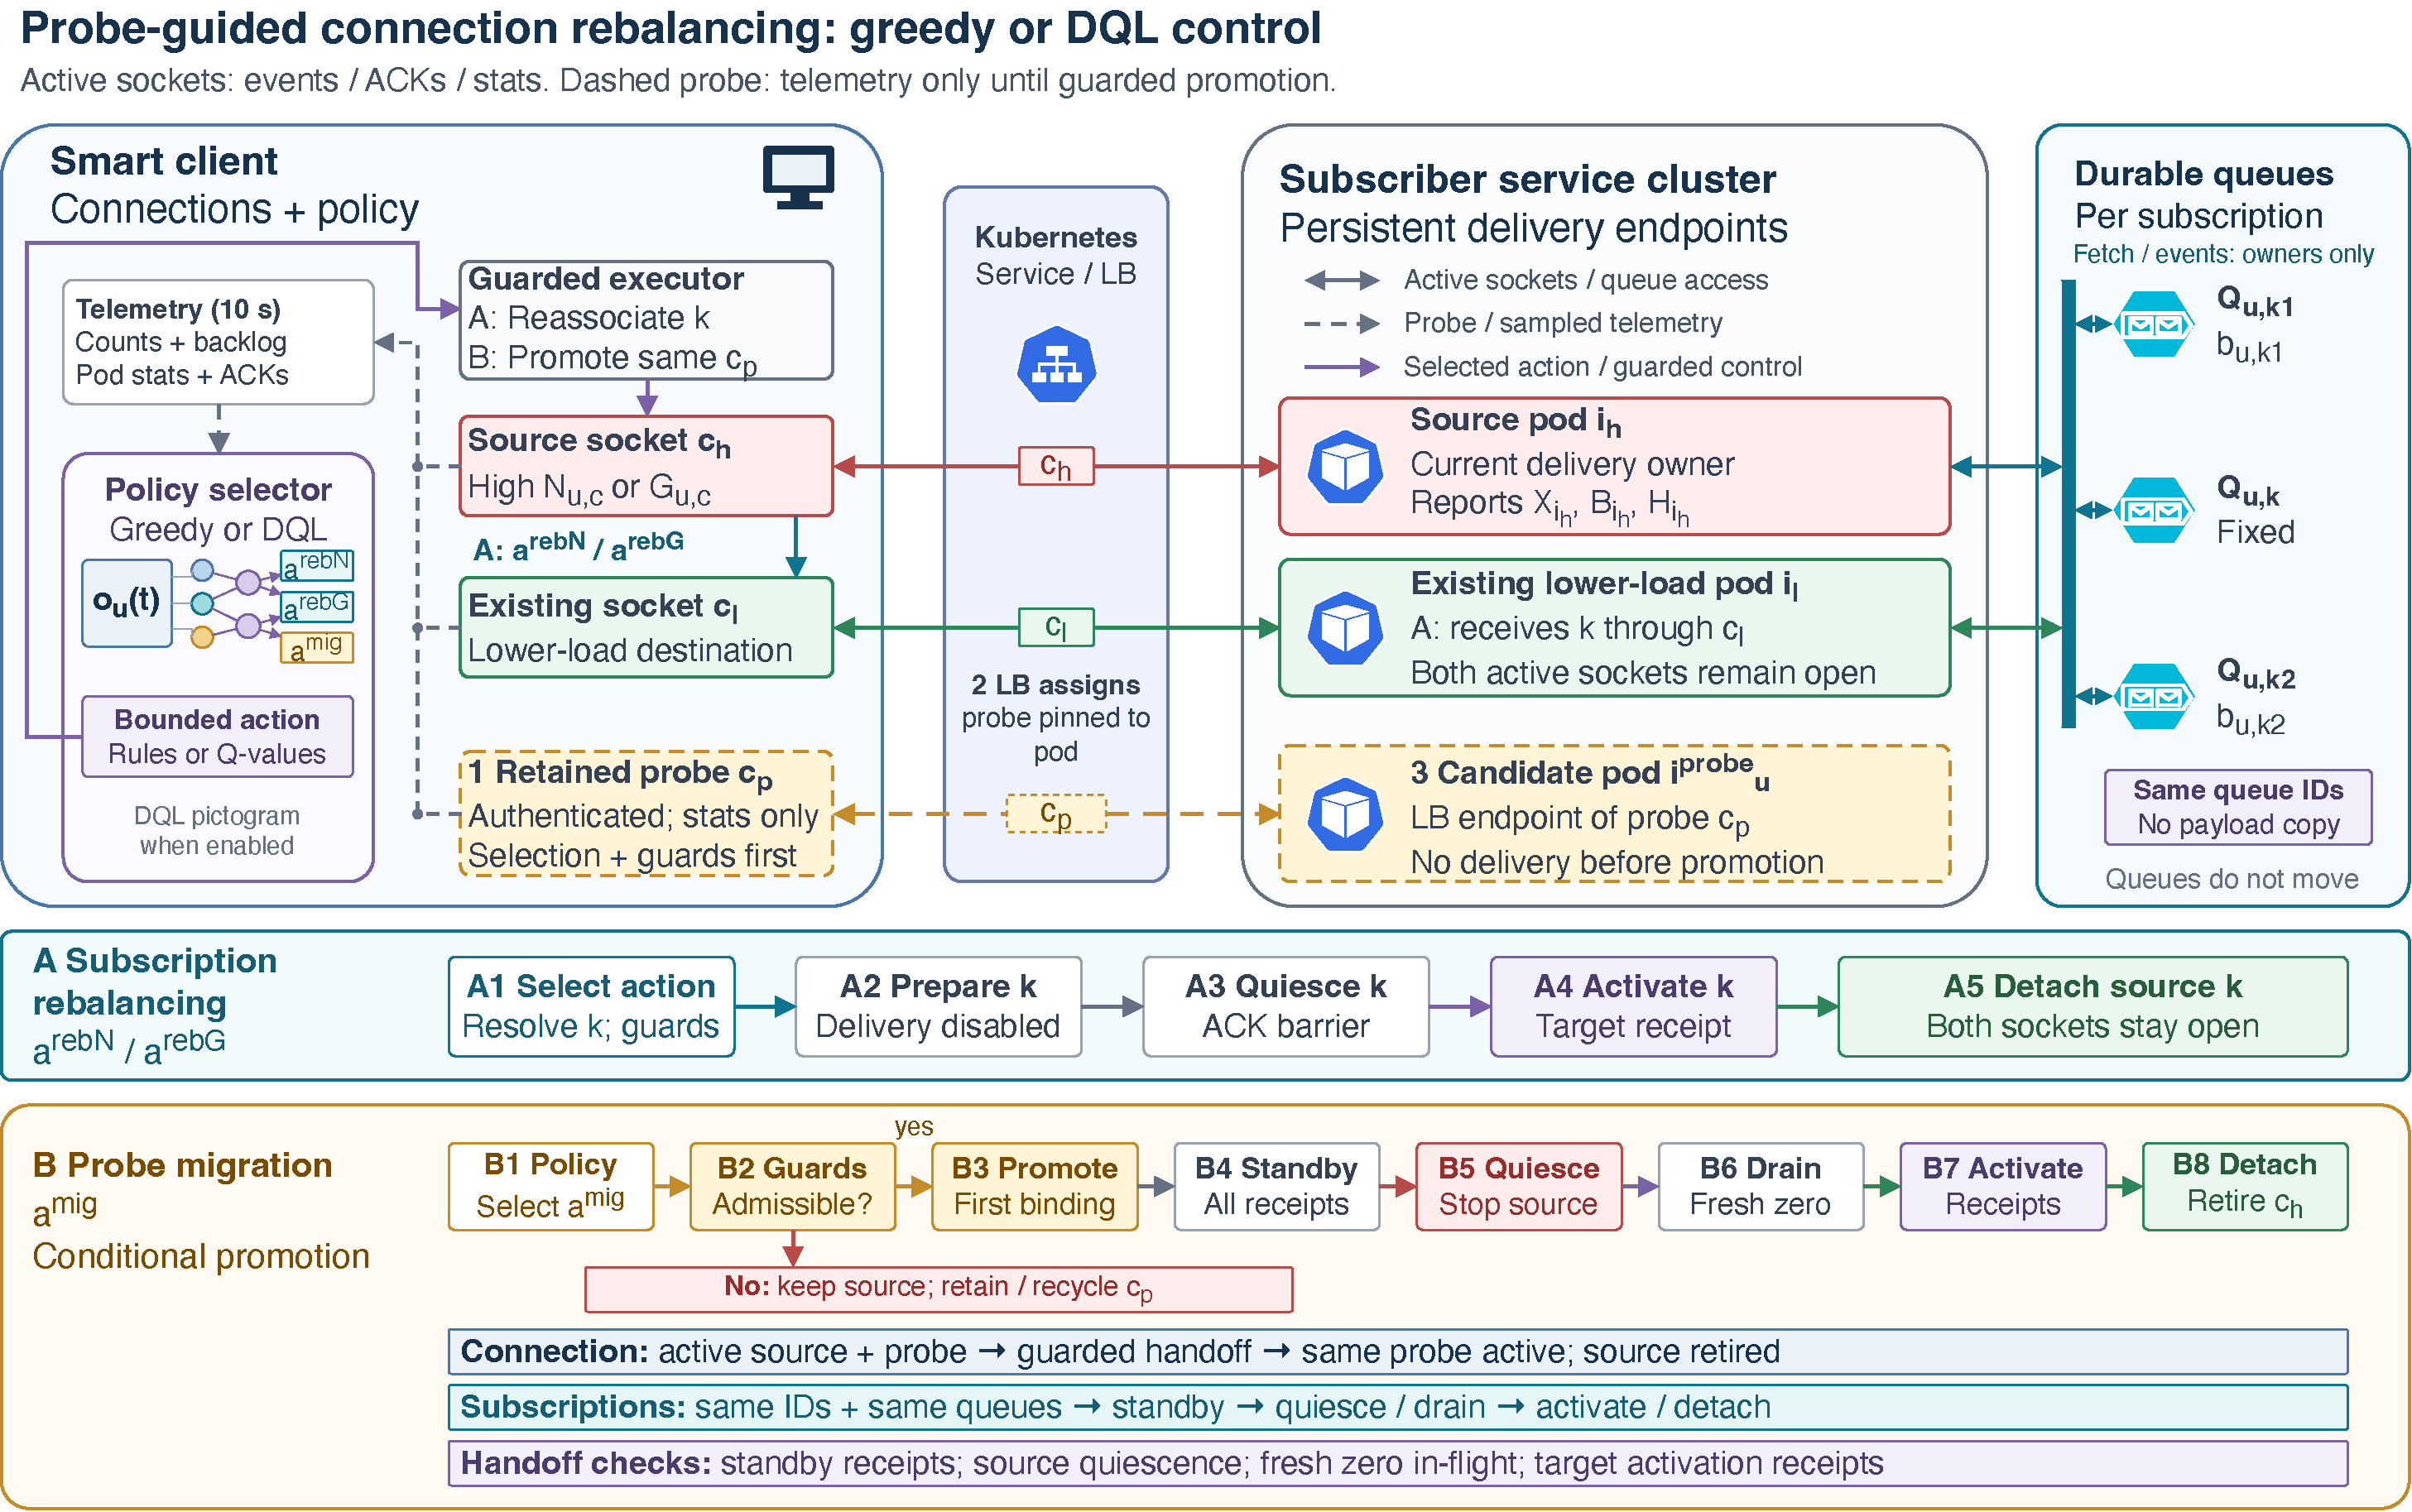
\includegraphics[width=\linewidth,height=0.83\textwidth,keepaspectratio]{figures/control-architecture-original-style.pdf}
	\caption{Shared probe-guided architecture with greedy or DQL selection. Path A rebalances subscriptions between existing sockets. Path B promotes the retained probe through its first standby binding, waits for all standby receipts, quiesces and drains the source, activates the target, detaches the source bindings, and retires the old socket. Unselected sockets and durable queues remain in place. The DQL pictogram denotes the optional learned selector, not an additional handoff service.}
	\Description{Two-path architecture with clients, subscriber Pods, and durable queues. Active and probe telemetry feed a greedy or DQL selector and a shared guarded executor. The selected probe keeps its load-balanced endpoint. Standby receipts, source quiescence, fresh zero-in-flight telemetry, activation receipts, and source detachment govern handoff. No ownership registry or epoch-commit service is shown.}
	\label{fig:control_architecture}
\end{figure}
\end{landscape}
}

\section{Problem Formulation}
\label{sec:problem-formulation}

The main quantities are client subscriptions $\mathcal{K}_u$, active sockets
$\mathcal{C}_u$, per-subscription backlog $b_{u,k}$, and the corresponding
connection loads $(N_{u,c},G_{u,c})$. Pod-wide quantities $(X_i,B_i)$ include
all clients served by Pod $i$. Appendix~\suppref{app:notation} collects the full
symbol reference; definitions also appear at their first use below.

We model the system at discrete control epochs $t=0,1,\ldots,T$. The interval
between adjacent epochs is $\Delta$ seconds: the next epoch is $t+1$, while
its physical time is $(t+1)\Delta$. Live-event timestamps and durations are
reported separately in seconds. Let
$\mathcal{S}=\{1,\ldots,n\}$ be the set of subscriber pods and
$\mathcal{U}=\{1,\ldots,m\}$ be the set of clients. Client $u$ maintains a
subscription set $\mathcal{K}_u(t)$ and a set of persistent transport
connections $\mathcal{C}_u(t)$, with
$1\leq |\mathcal{C}_u(t)|\leq C_{\max}$.
Indices $i,u,c,k$ refer to Pods, clients, connections, and subscriptions,
respectively. Calligraphic symbols denote sets; their cardinalities are
counts. In the single-client scaling rules, $C(t)=|\mathcal{C}_u(t)|$ and
$N_{\mathrm{sub}}(t)=|\mathcal{K}_u(t)|$ are count shorthands with the fixed client
index suppressed. They are never used as sets. Figure labels and algorithm
steps may omit $(t)$ when all quantities refer to the same decision epoch.

\subsection{Per-Subscription Queues}

Each subscription has a queue that stores messages waiting to be delivered and
processed. Let $Q_{u,k}(t)$ be the queue of subscription
$k\in\mathcal{K}_u(t)$, and let
\begin{equation}
	b_{u,k}(t)=|Q_{u,k}(t)|
\end{equation}
be the backlog for that subscription. This is the basic backlog measure used
by the client. At the pod level, backlog is a
server-owned aggregate. Let $\mathcal{R}_i(t)$ denote the set of subscription
queues currently served by pod $i$, and let $\tilde{b}_{i,r}(t)$ be the backlog
of server-side subscription queue $r\in\mathcal{R}_i(t)$. If queue $r$
corresponds to client $u$ and subscription $k$, then $\tilde{b}_{i,r}(t)$ is
the server-side counterpart of $b_{u,k}(t)$; however, $\mathcal{R}_i(t)$ also
contains queues belonging to other clients and is maintained by the pod, not by
any single client.

Let $z_{u,k,c}(t)\in\{0,1\}$ indicate whether subscription $k$ of client $u$ is
assigned to connection $c\in\mathcal{C}_u(t)$. Feasible assignment requires
\begin{equation}
	\sum_{c\in\mathcal{C}_u(t)} z_{u,k,c}(t)=1,
	\qquad \forall u,\; k\in\mathcal{K}_u(t).
	\label{eq:subscription_assignment}
\end{equation}
Let $i_{u,c}(t)\in\mathcal{S}$ denote the pod index reached by connection
$c$. This endpoint mapping differs from the Pod name $p_i$ and from the
selected DQL action $a_u(t)$.
The number of subscriptions and cumulative subscription backlog on connection
$c$ are
\begin{align}
	N_{u,c}(t) &= \sum_{k\in\mathcal{K}_u(t)} z_{u,k,c}(t),\\
	G_{u,c}(t) &= \sum_{k\in\mathcal{K}_u(t)}
	b_{u,k}(t)z_{u,k,c}(t).
	\label{eq:connection_backlog}
\end{align}
The first term captures subscription-management pressure on the connection; the
second captures queue pressure induced by the subscriptions mapped to that
connection.

\subsection{Pod Statistics and Partial Observability}

Each pod exposes a statistics tuple through active connections and probe
connections:
\begin{equation}
	y_i(t)=\bigl(p_i,\; X_i(t),\; B_i(t),\; H_i\bigr),
	\label{eq:pod_stats}
\end{equation}
Here $p_i$ is the pod name, and $X_i(t)$ is its subscription count.
The value $B_i(t)$ is the cumulative backlog across all subscription queues
served by pod $i$. The value $H_i$ is the configured maximum processing threshold. Using the
server-side queue set $\mathcal{R}_i(t)$, the pod-level subscription count and
cumulative pod backlog are
\begin{equation}
	X_i(t)=|\mathcal{R}_i(t)|,\qquad
	B_i(t)=
	\sum_{r\in\mathcal{R}_i(t)}
	\tilde{b}_{i,r}(t).
	\label{eq:pod_backlog}
\end{equation}
Thus $B_i(t)$ is not defined by summing over the connection set
$\mathcal{C}_u(t)$ of a particular client. A client's connections determine
which pod statistics it can observe and which subscriptions it can move, but
the pod backlog itself is the cumulative backlog over all subscription queues
served by that pod. These pod-level values include traffic from many clients
and are not directly computable by a single client unless reported by the pod.

At each statistics interval $\Delta$ (10 seconds in the target deployment),
every active connection receives the tuple of its current pod. In addition,
client $u$ maintains one authenticated probe connection whose endpoint is
selected by the load balancer and receives its tuple. The client
retains the probe socket and its endpoint identity until promotion, expiry, or
recycling; it does not resample a different pod merely by reading the next
observation. Therefore the client observes only a subset
$\mathcal{O}_u(t)\subseteq\mathcal{S}$ of pod states:
\begin{equation}
	\mathcal{O}_u(t)=
	\{i_{u,c}(t):c\in\mathcal{C}_u(t)\}
	\cup
	\{i^{\mathrm{probe}}_u(t)\}.
\end{equation}
The client stores the newest tuple for each observed pod in a local cache. This
makes the placement problem partially observable: global cluster variance is
available to an offline evaluator or simulator, but not to an individual client
controller. In particular, an admissible migration target must be represented
by a currently retained probe socket; the client cannot replace the sampled
candidate with an unobserved globally optimal pod.

\begin{assumption}[Available deployment signals]
For every pod $i$ observed by client $u$, where $i\in\mathcal{O}_u(t)$, the
protocol supplies $(p_i,X_i(t),B_i(t),H_i)$ in a statistics frame, header, or
control message. Client
$u$ can also measure its own per-subscription backlogs $b_{u,k}(t)$, delivered
message count, processed message count, acknowledged message count, active
connection count, and migration count over each interval $\Delta$.
\end{assumption}

\begin{assumption}[Transport abstraction]
The underlying transport is required only to maintain long-lived client--pod
connections, multiplex one or more subscriptions over a connection, support
subscription migration or reassignment, and expose periodic statistics through
headers, frames, or control messages. STOMP-over-TCP, custom TCP streams, and
WebSocket-based messaging are concrete examples of this abstraction.
\end{assumption}

\begin{remark}
The pod threshold $H_i$ is not treated as an actual drain rate. The true drain
rate depends on the queue subsystem, pod scheduling, network transport,
connection behavior, client processing capacity, and acknowledgement rate.
Hence $B_i(t)/(H_i\Delta+\varepsilon_0)$ is used only as a dimensionless
pod-side pressure ratio. Here $B_i$ counts messages, $H_i$ has units of
events per second, and $\varepsilon_0$ has units of messages. The ratio is
not an estimate of the actual drain time.
\end{remark}

\subsection{Local Imbalance Measures}

For client $u$, define the mean subscription count and mean backlog load across
its own connections:
\begin{align}
	\bar{N}_u(t)
	&= \frac{1}{|\mathcal{C}_u(t)|}
	\sum_{c\in\mathcal{C}_u(t)} N_{u,c}(t),\\
	\bar{G}_u(t)
	&= \frac{1}{|\mathcal{C}_u(t)|}
	\sum_{c\in\mathcal{C}_u(t)} G_{u,c}(t).
\end{align}
The corresponding variances are
\begin{align}
	V^N_u(t)
	&= \frac{1}{|\mathcal{C}_u(t)|}
	\sum_{c\in\mathcal{C}_u(t)}
	\bigl(N_{u,c}(t)-\bar{N}_u(t)\bigr)^2,\\
	V^G_u(t)
	&= \frac{1}{|\mathcal{C}_u(t)|}
	\sum_{c\in\mathcal{C}_u(t)}
	\bigl(G_{u,c}(t)-\bar{G}_u(t)\bigr)^2.
\end{align}
The first variance captures subscription-management skew, while the second
captures backlog skew. The local rebalancing objective is therefore
\begin{equation}
	V_u(t)=
	\eta_N\widehat{V}^N_u(t)
	+\eta_G\widehat{V}^G_u(t),
	\qquad
	\eta_N+\eta_G=1,
	\label{eq:local_connection_imbalance}
\end{equation}
where hats denote normalized quantities. This formulation is necessary because
two connections can have equal backlog but very different subscription counts,
or equal subscription counts but very different backlog.
The normalized terms place the two variances on a common scale before they are
combined. In the evaluation setup, we use positive reference values
$V^N_{\mathrm{ref}}$ and $V^G_{\mathrm{ref}}$ and compute
\begin{align*}
	\widehat{V}^N_u(t)
	&=\min\left\{\frac{V^N_u(t)}{V^N_{\mathrm{ref}}},1\right\},\\
	\widehat{V}^G_u(t)
	&=\min\left\{\frac{V^G_u(t)}{V^G_{\mathrm{ref}}},1\right\}.
\end{align*}
Thus $V_u(t)$ is a dimensionless connection-imbalance score in which the
subscription-count component and the backlog-load component are comparable.
The weights $\eta_N,\eta_G\geq0$ determine how much the controller prioritizes
subscription-management fairness versus backlog-load fairness. For example,
larger $\eta_N$ makes the controller more sensitive to connections carrying
too many subscriptions, while larger $\eta_G$ makes it more sensitive to
connections accumulating more queued messages. The constraint
$\eta_N+\eta_G=1$ makes $V_u(t)$ a convex combination rather than an
unbounded sum.

\subsection{Pod Pressure and Deployable Reward}

For an observed pod $i\in\mathcal{O}_u(t)$, define normalized pressure terms
\begin{align}
	P^X_i(t) &= \min\left\{\frac{X_i(t)}{X_{\mathrm{safe}}},1\right\},\\
	P^B_i(t) &= \min\left\{\frac{B_i(t)}{B_{\mathrm{ref}}},1\right\},\\
	P^H_i(t) &= \min\left\{\frac{B_i(t)}{H_i\Delta+\varepsilon_0},1\right\},
	\qquad \varepsilon_0>0.
\end{align}
Here $X_{\mathrm{safe}}$ is the subscription count at which pod reliability begins to
degrade. The value $X_{\mathrm{hard}}$ is the hard reference count at which we treat the
pod as severely overloaded by subscription-management work.
The value $B_{\mathrm{ref}}$ is the backlog reference used for normalization. The condition
$X_{\mathrm{hard}}>X_{\mathrm{safe}}$ is required. Since high subscription count has been
observed to make connections unreliable, we also define a nonlinear
reliability-risk penalty
\begin{equation}
	P^R_i(t)=
	\left[
	\frac{X_i(t)-X_{\mathrm{safe}}}
	{X_{\mathrm{hard}}-X_{\mathrm{safe}}}
	\right]_+^2,
	\qquad [x]_+=\max\{x,0\}.
\end{equation}
The pod pressure score is
\begin{align}
	P_i(t)=
	&\omega_X P^X_i(t)
	+\omega_B P^B_i(t) \nonumber\\
	&+\omega_H P^H_i(t)
	+\omega_R P^R_i(t),
	\label{eq:pod_pressure}\\
	&\sum_{q\in\{X,B,H,R\}}\omega_q=1,\qquad \omega_q\geq 0. \nonumber
\end{align}
Here $P^X_i(t)$ measures normalized subscription-count pressure.
The term $P^B_i(t)$ measures normalized cumulative-backlog pressure.
The term $P^H_i(t)$ measures backlog pressure relative to the processing threshold.
Finally, $P^R_i(t)$ measures nonlinear reliability risk and becomes active only
when $X_i(t)>X_{\mathrm{safe}}$. The coefficients
$\omega_X,\omega_B,\omega_H,\omega_R$ specify how much importance the policy
assigns to each pressure component. For example, if subscription-heavy pods are
known to become unreliable before backlog becomes large, then $\omega_X$ and
$\omega_R$ receive greater weight than $\omega_B$ and $\omega_H$. If queue
accumulation is the dominant failure mode, $\omega_B$ and $\omega_H$
receive greater weight. This score keeps subscription count and backlog
count as distinct load dimensions.

Client $u$ also computes local backlog and backlog-growth pressure:
\begin{align}
	B_u(t) &= \sum_{k\in\mathcal{K}_u(t)} b_{u,k}(t),\\
	\mathrm{Grow}_u(t) &= \bigl[B_u(t)-B_u(t-1)\bigr]_+,\qquad t\geq1.
\end{align}
At initialization, $\mathrm{Grow}_u(0)=0$. Let $T_u(t)$ be the effective client-side
throughput in events per second. The rates $T^{\mathrm{del}}_u(t)$, $T^{\mathrm{proc}}_u(t)$,
and $T^{\mathrm{ack}}_u(t)$ are the delivered, processed, and acknowledged counts in
the measured interval, each divided by its duration $\Delta$:
\begin{equation}
	T_u(t)=
	\min\{T^{\mathrm{del}}_u(t),T^{\mathrm{proc}}_u(t),T^{\mathrm{ack}}_u(t)\}.
\end{equation}
For an action that selects or keeps pod $i$, the deployable reward is
\begin{align}
	R_u(t)=
	&-\lambda_1\widehat{B}_u(t)
	-\lambda_2\widehat{\mathrm{Grow}}_u(t)
	-\lambda_3 P_i(t)
	-\lambda_4 V_u(t) \nonumber\\
	&-\lambda_5 M_u(t)
	-\lambda_6\widehat{C}_u(t)
	+\lambda_7\widehat{T}_u(t),
	\label{eq:deployable_reward}
\end{align}
where $M_u(t)$ is the migration indicator or normalized migration count,
$\widehat{C}_u(t)=|\mathcal{C}_u(t)|/C_{\max}$, and
$\lambda_\ell\geq0$ with $\sum_{\ell=1}^{7}\lambda_\ell=1$.
The hats on backlog, backlog growth, and throughput denote their normalized
versions under the stated experiment's scaling convention, not different
physical quantities. This reward is computable by the client from
local measurements and observed pod tuples.

Detailed reference-scale calibration, the global evaluation objective, and
step-by-step proofs of the subscription-density and backlog-variance
properties are provided in Section~\suppref{app:extended-mathematics}. The full notation reference is in
Section~\suppref{app:notation}.

\section{Policy Selection and Guarded Rebalancing}
The framework places a policy selector above three concrete runtime mechanisms:
pod migration, client-side connection scaling, and subscription redistribution
across active connections. These mechanisms solve different parts of the same
load-distribution problem. Migration changes where a connection terminates,
scaling changes how much parallelism the client maintains, and rebalancing
changes how subscriptions use that parallelism. Keeping the mechanisms
separate makes each action deployable, while the selected policy decides which
action is appropriate at a given control epoch.

The separation between reward and feasibility is deliberate. Safe-RL research
distinguishes performance optimization from constraint satisfaction
\cite{Gu2024SafeRL}; a migration penalty alone cannot enforce ownership or
readiness. Krasowski et al. distinguish action masking, replacement, and
projection as intervention mechanisms \cite{Krasowski2023ProvablySafe}.
Our masks and execution-time checks restrict the deployable actions, but do
not confer the formal safety guarantees of a verified environment model.

\subsection{Greedy and Learned Policy Roles}
Both policy families use the client-visible measurements and deterministic
execution checks defined above. In the scale-out study, the guarded-greedy
selector requests $a^{\mathrm{mig}}$ whenever that action is admissible and
otherwise stays. Its guard assesses projected source and target pressure
after moving the selected subscription group, so a lightly subscribed but
heavily backlogged candidate need not be accepted. The source-selection and
pressure checks are shared with DQL; they are not learned from DQL's outcomes.

The mixed-workload study uses a different deterministic comparator, labelled
\emph{Heuristic}: it applies threshold rules for subscription-count and backlog
imbalance as well as migration. The independent \emph{Scripted} timing controls
use pressure-unaware schedules and are sensitivity controls, not substitutes
for the stronger guarded-greedy comparison. Table~\ref{tab:policy-roles}
keeps these identities distinct.

\begin{table}[!htbp]
\centering\small
\caption{Policy roles and the comparison each supports. Greedy and DQL share
the rebalancing mechanism; the studies retain their original policy labels.}
\Description{Five policy rows distinguish pressure-aware greedy migration,
the multidimensional heuristic, DQL, random scripted schedules, and unchanged placement.}
\label{tab:policy-roles}
\begin{tabular}{p{0.19\textwidth}p{0.39\textwidth}p{0.32\textwidth}}
\toprule
Policy & Decision rule & Evidence role\\
\midrule
Guarded-greedy & Promote an admissible pressure-improving probe & Strong non-learning scale-out control\\
Heuristic & Threshold rules over count, backlog, and placement & Non-learning multi-objective comparator\\
Frozen DQL & Masked maximum learned action value; no evaluation updates & Learned multi-objective selector\\
Scripted schedules & Fixed or jittered timing; random source and target & Pressure-unaware sensitivity controls\\
Static / scale-out only & Retain established connection assignment & No-rebalancing reference\\
\bottomrule
\end{tabular}
\end{table}

The shared contribution is probe-guided actuation, not the invention of either
greedy search or Q-learning. The experiments compare policy choices without
feeding DQL's holdout decisions back into the scripted rules. Learning traces
can inform separate development work, but automatic DQL-to-script tuning is
not part of the evaluated system.
\subsection{DQL State, Action, and Value Function}

The client-side controller is modeled as a partially observable sequential
decision problem. At each control epoch, client $u$ constructs an observation
vector
\begin{equation}
	o_u(t)=
	\left[
	o^B_u(t),o^N_u(t),o^G_u(t),o^C_u(t),o^P_u(t),o^D_u(t)
	\right],
	\label{eq:dql_observation}
\end{equation}
where $o^B_u(t)$ contains normalized local backlog and backlog growth.
The branch $o^N_u(t)$ describes subscription-count imbalance using terms such as
$N_{u,c}(t)$ and $V^N_u(t)$. The branch $o^G_u(t)$ describes backlog imbalance
using terms such as $G_{u,c}(t)$ and $V^G_u(t)$.
The branch $o^C_u(t)$ contains connection count and effective throughput.
The branch $o^P_u(t)$ contains pressure, subscription count, and cumulative
backlog for the current and probe pods. Finally, $o^D_u(t)$ contains cooldown
and statistics-staleness features. For current-pod features, $c^\star$ denotes
the connection being evaluated. All quantities are normalized before they
enter the Q-network.

The DQL action space is defined using bounded action templates rather than all
possible subscription assignments, which keeps the decision problem tractable:
\begin{equation}
	\mathcal{A}=
	\{a^{\mathrm{stay}},a^{\mathrm{reb}N},a^{\mathrm{reb}G},a^{\mathrm{scale}+},a^{\mathrm{scale}-},a^{\mathrm{mig}}\}.
	\label{eq:dql_actions}
\end{equation}
Here $a^{\mathrm{stay}}$ makes no change. The action $a^{\mathrm{reb}N}$ moves one subscription
from the connection with the most subscriptions to the one with the fewest.
The action $a^{\mathrm{reb}G}$ moves the subscription with the largest predicted decrease
in backlog variance. The action $a^{\mathrm{scale}+}$ opens one new connection and,
when allowed, makes bounded subscription moves toward the target $\Theta_N$.
The action $a^{\mathrm{scale}-}$ closes a subscription-free connection only if the
remaining connections meet the required capacity and observed backlog is zero.
The action $a^{\mathrm{mig}}$ requests promotion of the retained probe. It transfers the
evaluated connection or bounded subscription group only if the admissibility
and hysteresis conditions pass. The DQL network selects
the action template; it does not choose an arbitrary Pod or directly change a
subscription assignment. The deterministic executor computes the concrete
source connection, target connection, and subscription using the load-aware
rules in Algorithms~\suppref{alg:adaptive_parallel_scaling} and
\suppref{alg:connection_rebalancing}, and may reject an inapplicable template as a
guarded no-op.
Here $\Theta_N$ is the configured maximum desired subscription count per
connection, not the network parameter vector $\theta$.
The evaluated legacy checkpoint uses a compatible action profile; both
scaling actions are disabled in the loaded cluster trial. The later
cap-restoring scale-up contract is distinct. Table~\suppref{tab:action-contract-map}
retains these version boundaries and their evaluation scope.
DQL uses two action-value networks with the same architecture but different
roles. The online network $Q_\theta(o,a)$ is the trainable network used for
current action evaluation and epsilon-greedy action selection. The target
network $Q_{\theta^-}(o,a)$ is a delayed copy of the online network. It is not
used for selecting the live action and is not updated by every gradient step;
it is used only to compute a stable Bellman target for the next observation.
For a transition
$\xi_t=(o_u(t),a_u(t),R_u(t),o_u(t+1))$ sampled from replay buffer
$\mathcal{D}$, the target is
\begin{equation}
	y_t =
	R_u(t) + \gamma
	\max_{a'\in\mathcal{A}^{\mathrm{adm}}_u(t+1)}Q_{\theta^-}(o_u(t+1),a'),
	\label{eq:dql_target}
\end{equation}
where $\gamma\in[0,1)$ is the discount factor and $\theta^-$ denotes the target
network parameters. The set $\mathcal{A}^{\mathrm{adm}}_u(t+1)\subseteq\mathcal{A}$
contains the actions admitted by the next observation's execution guards;
an infeasible action cannot supply the bootstrap value. The equation applies
to non-terminal transitions. At a true terminal state, $y_t=R_u(t)$.
An interrupted observation window is not assigned an artificial terminal
reward. The online network parameters $\theta$ are trained by
minimizing
\begin{equation}
	\mathcal{L}(\theta)=
	\mathbb{E}_{\xi_t\sim\mathcal{D}}
	\left[
	\left(y_t-Q_\theta(o_u(t),a_u(t))\right)^2
	\right].
	\label{eq:dql_loss}
\end{equation}
Every $K_{\mathrm{sync}}$ training updates, the target network is synchronized by copying the
online parameters, $\theta^- \leftarrow \theta$. This separation prevents the
same rapidly changing network from defining both the prediction
$Q_\theta(o_u(t),a_u(t))$ and the target $y_t$. The parameters $\theta$ and
$\theta^-$ contain all network weights and biases; $\Theta_N$ is instead a
subscription-count threshold. The learning rate $\alpha$ controls the update
$\theta\leftarrow\theta-\alpha\nabla_\theta\mathcal{L}(\theta)$ and is
distinct from the imbalance weights $\eta_N,\eta_G$.
This formulation makes rebalancing a sequential control problem: a migration,
new connection, or subscription move can reduce future backlog but may incur
immediate migration or connection cost.

\begin{table}[!htbp]
\centering\small
\caption{Configuration of the v3 DQL policy used in the reported holdout,
scale-out simulator, and October live trial. Later learner variants are
reported separately in Appendix~\suppref{app:action-diagnostics}.}
\Description{A reproducibility table of network dimensions, training settings,
reward weights, exploration, and frozen evaluation settings.}
\label{tab:dql-configuration}
\begin{tabular}{p{0.38\textwidth}p{0.54\textwidth}}
\toprule
Setting & Value\\
\midrule
Network; optimizer & Dense 21--32--6; ReLU hidden, linear output; mini-batch gradient descent\\
Discount; learning rate & $\gamma=0.99$; $\alpha=0.001$\\
Replay; batch; target copy & Uniform replay, capacity 5,000; batch 16; copy every 250 updates\\
Bootstrap; loss & Target-network maximum over admitted actions; squared TD error\\
Training budget & 10,000 transitions per candidate; 9,985 updates after batch warm-up\\
Training exploration & $\epsilon_0=1$, multiplier $\exp(\log(0.05)/10{,}000)$; floor 0.05\\
Reward weights $(\lambda_1,\ldots,\lambda_7)$ & $(0.20,0.15,0.20,0.15,0.10,0.05,0.15)$\\
Pressure weights $(\omega_X,\omega_B,\omega_H,\omega_R)$ & $(0.30,0.25,0.20,0.25)$\\
Imbalance weights & $\eta_N=\eta_G=0.5$\\
Frozen evaluation & $\epsilon=0$; no model or replay updates; checkpoint hash retained\\
\bottomrule
\end{tabular}
\end{table}

\subsection{Shared Control Loop}
Algorithm~\ref{alg:compact-control} summarizes the policy-independent runtime.
The full sizing and rebalancing executors and the DQL training loop are
retained in Section~\suppref{app:runtime-details}.

\begin{algorithm}[!htbp]
\small
\caption{Probe-Guided Selection and Guarded Execution}
\label{alg:compact-control}
\SetKwInOut{Input}{Input}
\Input{Active connections, retained probe, declared policy and action profile}
\While{client is active}{
 Read active/probe telemetry and client queue/ACK counters\;
 Construct observation and freshness, capacity, cooldown and handoff masks\;
 Select an admitted action using the declared greedy or DQL policy\;
 Recheck guards before applying the selected action\;
 \eIf{migration is selected and admitted}{
  Prepare standby bindings on the same probe; await receipts\;
  Quiesce the source; wait for fresh zero-in-flight telemetry\;
  Activate target bindings; detach source bindings; retire the source socket\;
  Retain unselected sessions and replenish the empty probe\;
 }{
  Execute the admitted bounded rebalancing/scaling action, or stay\;
 }
 Record the applied action, observed reward and guard outcome\;
 Update learning state only in a declared training run with a valid transition\;
}
\end{algorithm}
\subsubsection{Exploration, Hysteresis, and Migration}

Let $\mathcal{A}^{\mathrm{adm}}_u(t)\subseteq\mathcal{A}$ contain only the templates
that pass the current freshness, capacity, cooldown, and handoff guards. The
DQL policy uses epsilon-greedy exploration over this masked set:
\begin{equation}
	a_u(t)=
	\begin{cases}
		\text{Uniform}(\mathcal{A}^{\mathrm{adm}}_u(t)), & \text{w.p. } \epsilon,\\
		\arg\max_{a\in\mathcal{A}^{\mathrm{adm}}_u(t)} Q_\theta(o_u(t),a), & \text{w.p. } 1-\epsilon.
	\end{cases}
\end{equation}
The exploration probability decreases during training. Frozen validation and
deployment policies use $\epsilon=0$. This prevents unreviewed exploratory
changes during evaluation. Online exploration would require a separate
safety study. Migration is
executed only when the selected action is $a^{\mathrm{mig}}$ and the retained probe
candidate improves the estimated value by a hysteresis threshold:
\begin{equation}
	Q_\theta(o_u(t),a^{\mathrm{mig}}) >
	Q_\theta(o_u(t),a^{\mathrm{stay}})+\delta.
\end{equation}
This threshold prevents oscillatory migrations caused by small or stale
statistical differences. It does not choose the probe endpoint: the Kubernetes
load balancer already fixed that endpoint when the probe socket was opened.
Passing this value test is necessary but not sufficient. The executor also
checks telemetry freshness, target capacity, source--target separation, cooldown,
and the absence of a conflicting handoff. As a result, most probes
can remain telemetry-only and may expire or be recycled without carrying a
subscription.

The exact network input order, normalization constants, and deterministic
comparator thresholds are retained in Section~\suppref{app:feature-order}. Checkpoint persistence and full execution
details are in Section~\suppref{app:runtime-details}.

\section{Oracle Cloud Cluster Deployment Experiment}
\label{sec:mumbai-experiment}

We deployed the connection-replacement mechanism in an Oracle Cloud cluster
running Kubernetes in a development environment and first exercised it with 20,000
registered subscriptions. This initial experiment
measures live probe promotion, subscription reassociation, handoff timing, and
post-migration topology. The controlled scale-out and policy comparisons in
Section~\ref{sec:locked-evidence} use a simulator and are reported separately.
Sections~\suppref{sec:mumbai-startup} and~\ref{sec:live-dql-scaleout} report
separate isolated trials, including selective DQL migration during delivery
and a one-to-four-Pod scale-out sequence.

\subsection{Deployment and Execution}

The deployment contained ten subscriber-service pods. Ten client processes
each maintained five active persistent connections, with 400 subscriptions per
connection, and one additional subscription-free probe. The inventory had
four event-type groups, each with 5,000 subscriptions. Every client loaded the
same frozen DQL checkpoint, with exploration disabled and no training updates
during evaluation. The deployed action profile admitted rebalancing and
migration but masked connection scale-up and scale-down.

Each client could execute at most one guarded connection migration. A selected
probe was promoted only after telemetry and execution checks passed. The
executor then reassociated the source connection's 400 subscriptions, drained
in-flight delivery, retired the source socket, and opened a fresh
subscription-free probe. Subscription receipts and server-reported counts
were checked against the client assignment. After execution, each process
held its topology for 1,800 seconds and checked it again before shutdown.
The statistical unit is one deployment run, containing ten client migrations.

\begin{table}[t]
  \caption{Measured Oracle Cloud cluster deployment results. Handoff and drain statistics
  summarize ten executed connection migrations. Drain wait is part of handoff
  time, not an additional independent interval.}
  \Description{Live experiment with ten pods, twenty thousand subscriptions,
  ten successful connection replacements, four thousand moved subscriptions,
  and exact final topology in all ten clients. Handoff median is 14.498 seconds;
  drain-wait median is 7.347 seconds.}
  \label{tab:mumbai-live-results}
  \centering
  \small
  \begin{tabular}{p{0.60\linewidth}r}
    \toprule
    Measurement & Observed value \\
    \midrule
    Subscriber-service pods / client processes & 10 / 10 \\
    Registered and attached subscriptions & 20,000 \\
    Active persistent connections / probes & 50 / 10 \\
    Executed full-connection migrations & 10 \\
    Subscriptions moved per migration / total & 400 / 4,000 \\
    Handoff time: minimum / median / maximum (s) & 7.898 / 14.498 / 101.563 \\
    Drain wait: minimum / median / maximum (s) & 1.264 / 7.347 / 92.450 \\
    Exact final topologies after 1,800 s & 10/10 \\
    Recorded deliveries / processed and acknowledged & 114,986 / 113,149 \\
    Processing failures / ACK failures / NACK failures & 0 / 0 / 0 \\
    Recorded duplicate candidates & 0 \\
    Independent pod samples / collection errors & 310 / 0 \\
    Pod restart increase during observation & 0 \\
    \bottomrule
  \end{tabular}
\end{table}

\subsection{Observed Handoff and Topology}

Table~\ref{tab:mumbai-live-results} shows that all ten clients replaced one
active connection and moved its full subscription set. In every case, the
destination was the retained probe, the other four active connections remained
in place, and the replacement probe had no subscriptions. The final checks
confirmed all 2,000 subscriptions and five active connections in each client
after the 30-minute hold. Thus, 4,000 subscriptions changed their transport
association while the complete 20,000-subscription client population remained
accounted for.

Handoff duration ranged from 7.898 to 101.563 seconds, with a median of
14.498 seconds. The corresponding source-drain waits ranged from 1.264 to
92.450 seconds, with a median of 7.347 seconds. The range is important:
replacement time includes waiting for outstanding work, not just opening
a socket. This run deliberately used eight processing workers
and a two-second processing delay per event in each client. Those settings
exercise handoff under a bounded client drain rate. The endpoint is handoff
behavior under this processing limit, rather than maximum Pod throughput.

The paired handoff/drain distributions and their statistical interpretation
are retained in Section~\suppref{app:cloud-timing}.
An independent collector retained 31 observations of each of the ten pods
over approximately 2,422 seconds. All pods remained Ready, with unchanged
pod, image, and process identities and no restart increase. These observations
establish operational continuity over this observation period. Long-term
availability is outside the measurement window.

\subsection{Event Accounting and Interpretation}

The clients recorded 114,986 deliveries and 113,149 processed and acknowledged
events, with no recorded processing, acknowledgement, or negative-
acknowledgement failures. The final difference is 1,837 deliveries whose
eventual status is not resolved by these counters. Zero duplicate candidates
describes the configured observation window, rather than an exactly-once
delivery guarantee. The run consumed existing queued work without a matched
static-policy workload. Its contribution is measured probe-based connection
replacement with 20,000 subscriptions: subscription reassociation, source
retirement, and the connection layout after the hold period. Its endpoints
are handoff execution and topology retention, not a comparative backlog-drain
rate.

The private evidence archive retains the frozen-policy and inventory hashes,
per-client decision and topology records, delivery counters, and independent
pod observations. A recursive manifest covers 134 files; aggregate values in
Table~\ref{tab:mumbai-live-results} come from the active-execution gate and
pod-observation summaries, not from simulator output.
\subsection{Loaded DQL Migration During Pod Scale-Out}
\label{sec:live-dql-scaleout}

We next tested selective connection replacement during event delivery in a
separate Oracle Cloud cluster run. One client attached 1,000 registered
subscriptions to four persistent connections on one subscriber Pod, with
250 subscriptions per connection. The isolated deployment then grew from
one to four Ready Pods while the same client process remained running.
The second Pod became Ready before standby activation was released; the
third and fourth Pods were added during observation. The transport load
balancer assigned each empty probe to a Pod. The client used the retained
socket only when DQL selected migration and the execution guards passed.

The frozen checkpoint had 9,985 training updates and used $\epsilon=0$.
The trial allowed three executed actions in a configured 600-second window,
with a 60-attempt probe-discovery budget. Telemetry had to satisfy the
180-second age limit and 0.8 minimum backlog coverage. Each Pod requested
1.5 CPU cores and 4~GiB memory, with limits of three cores and 6~GiB.
The client used 32 workers and a fixed one-second processing delay to keep
work outstanding during handoff. This setting tests acknowledgement-aware
migration under a bounded client drain rate, rather than maximum Pod capacity.

Two bounded batches each published four synthetic source events. Each event
matched 5,000 registered subscriptions, including the client's 1,000-subscription
cohort. Thus, publication exposed the queue to 40,000 copies while the measured
cohort accounted for 8,000 delivery attempts. Capacity was checked before each
batch against the existing 400~MB limit, retaining an 80~MB reserve and prior
unreconciled publication costs. No queue purge or quota increase was used.

\begin{table}[!htbp]
  \centering
  \small
  \caption{Executed frozen-DQL handoffs in the loaded Oracle Cloud scale-out
  run. P1 is the initial Pod; P2 and P3 are added Pods. Drain time is included
  in total handoff time. These are three actions within one run.}
  \Description{Three handoffs each move 250 subscriptions and retain the other
  three active sessions. The first two move from P1 to P2; the third moves the
  first group again from P2 to P3. Total times are 97.555, 10.881 and 79.657 seconds.}
  \label{tab:live-dql-loaded-handoffs}
  \begin{tabular}{llrrrr}
    \toprule
    Action & Path & Subscriptions & Other sessions & Drain (s) & Total (s) \\
    \midrule
    H1 & P1 to P2 & 250 & 3 retained & 93.862 & 97.555 \\
    H2 & P1 to P2 & 250 & 3 retained & 8.339 & 10.881 \\
    H3 & P2 to P3 & 250 & 3 retained & 76.166 & 79.657 \\
    \bottomrule
  \end{tabular}
\end{table}

Table~\ref{tab:live-dql-loaded-handoffs} records actual policy execution, not
just a migration recommendation. The three observed differences between the
migration and stay Q-values were 1.7126, 1.2919 and 1.8201. Each migration was
admissible and selected by the frozen network. Before-and-after session maps
show that every handoff preserved the other three active connections. Two
original sessions remained unchanged throughout the run. The mechanism
therefore replaced selected connections without disconnecting the whole pool.

\begin{figure}[!htbp]
  \centering
  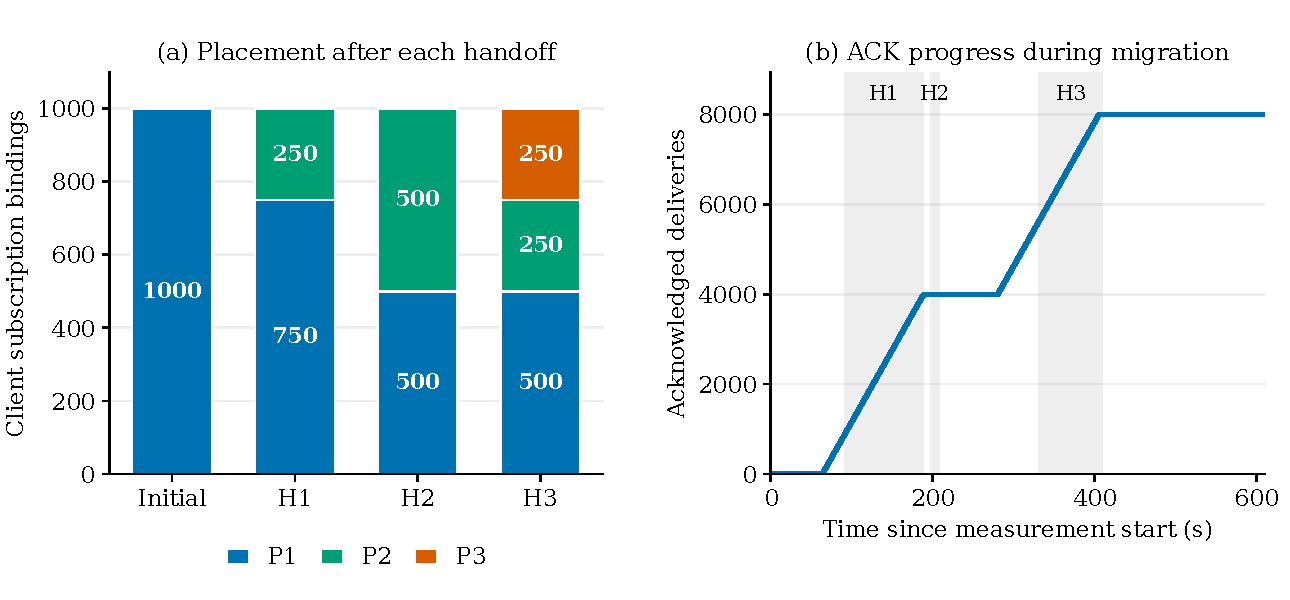
\includegraphics[width=\textwidth]{figures/live-dql-loaded-scaleout.pdf}
  \caption{Measured loaded DQL migration in the Oracle Cloud cluster.
  (a) Receipt-confirmed client bindings at the initial snapshot and after
  H1--H3. Each bar accounts for all 1,000 subscriptions; the four active
  connections each retain 250 subscriptions. P4 has no client bindings and
  is observed only through a probe. (b) Cumulative ACK receipts, aggregated
  in one-second bins. Shaded spans show the measured complete handoff
  intervals, including source drain. The curve describes this bounded
  workload, not a matched between-policy throughput comparison.}
  \Description{Placement changes from one thousand bindings on P1 to seven
  hundred fifty on P1 and two hundred fifty on P2, then five hundred on each,
  and finally five hundred on P1, two hundred fifty on P2 and two hundred fifty
  on P3. ACK receipts reach eight thousand while three shaded handoff intervals
  mark selective connection migration.}
  \label{fig:live-dql-loaded-scaleout}
\end{figure}

Figure~\ref{fig:live-dql-loaded-scaleout}(a) separates moved subscriptions
from handoff operations. H3 moves the group already transferred by H1, so
the three actions comprise 750 subscription-handoff operations involving
500 distinct subscriptions. The final distribution across the four available
Pods is 500, 250, 250 and zero. The maximum client population on one Pod falls
from 1,000 to 500, a 50\% reduction, without increasing the four active
connections. The last Pod remains a probe candidate after the three-action
budget is reached. Discovering it does not automatically promote it.

Figure~\ref{fig:live-dql-loaded-scaleout}(b) uses the confirmed ACK receipt
timestamp of each recorded delivery. Its cumulative total reaches 8,000,
and each of the 1,000 registered subscription hashes has eight acknowledged
delivery records. The ledger contains zero recorded ACK failures, processing
failures, duplicate candidates or unresolved deliveries at clean closure.
Long drain intervals remain visible: source retirement waits for outstanding
work instead of discarding it to shorten the measured handoff. The configured
window contains 60 decision records; its actual measurement boundaries span
609.716 seconds, including boundary handling.

The identity check uses STOMP message identifiers and confirms observed
delivery/ACK accounting. Source CloudEvent identities and individual backend
queue deletions are outside that ledger's scope. A separate unloaded
1,000-subscription run executed two handoffs in 5.244 and 5.172 seconds;
those timings are retained separately because the processing conditions
differ. The online and target weights remained identical to the input
checkpoint in both runs. The loaded run saved 39 valid experience transitions
without applying new training updates. The complete private archive verifies
256 files, and the manuscript figure uses identifier-free aggregates derived
from those records. The isolated deployment was restored to one Ready Pod;
all 13 shared-resource isolation checks passed.


\subsection{TTL Reconnection Comparison}
An isolated matched-preload pair used 5,000 subscriptions and 30,000 delivery
attempts per arm. Native TTL produced twelve server-matched interruptions and
26,831 confirmed ACKs (89.44\%), leaving 3,169 unresolved receipts. The
TTL-disabled DQL arm confirmed all 30,000 ACKs without interruptions, but its
telemetry guards held every decision at \emph{stay}. A 200-second minimum
telemetry sweep exceeded the 180-second freshness deadline. This pair measures
expiry-related interruption and receipt completion, not a learned-migration
throughput advantage. Unresolved receipts are not classified as event loss.

Detailed TTL implementation paths, recovery endpoints, the two-burst trial,
and matched-preload diagnostics are provided in
Section~\suppref{sec:ttl-reconnection}.
The separate 2,000-subscription calibration and startup-under-load trial is
retained in Section~\suppref{sec:mumbai-startup}.

\section{Experimental Method and Locked Simulator Evidence}
\label{sec:locked-evidence}

We evaluate recovery after subscriber-pod scale-out using 20,000 subscriptions,
ten persistent connections, and 775 million queued events. The primary
comparison measures the use of added pod capacity with guarded-greedy and
DQL-guided migration against retaining the initial connection placement. Supporting studies examine
multi-objective control, action selection, and adverse probe promotion.

\subsection{Recovery After Subscriber-Pod Scale-Out}
\label{sec:scaleout-recovery}

The primary recovery experiment models the capacity increase from one
subscriber pod to four. Ten persistent TCP connections are established on the
original pod, carrying 20,000 subscriptions. At the measurement boundary,
three additional ready pods provide processing capacity, while the ten
established connections retain their original endpoints. The comparison
therefore measures how effectively the client uses the added capacity through
probe promotion and subscription reassociation.

Four equal subscription groups begin with 100,000, 50,000, 5,000, and zero
queued events per subscription, respectively. The initial backlog is
$B(0)=775{,}000{,}000$ events. Round-robin assignment gives each connection
2,000 subscriptions and 77.5 million queued events. Consequently,
$V^N_u(0)=V^G_u(0)=0$: the initial bottleneck is concentrated pod placement.
This setup isolates whole-connection migration from pre-existing imbalance
between the client's connections.

The model assigns each pod a processing threshold of 100,000 events/s and
the client a base acknowledgement capacity of 250,000 events/s. Its bounded
connection-parallelism factor is three at ten connections. Service is limited
by both client capacity and each connection's share of its pod capacity.
The simulator's pressure-dependent service factor is
$\max\{0.35,1-0.42P_i^{\mathrm{sim}}\}$, where $P_i^{\mathrm{sim}}\in[0,1]$ is the simulator's
clipped load score, distinct from the deployable pressure in
(\ref{eq:pod_pressure}). These numerical rates define the simulator's service
assumptions rather than measured Pod benchmarks. Pressure is sampled before the action
and refreshed after the interval. For the clipped score, this service
multiplier lies in $[0.58,1]$: the model represents pressure-degraded service,
not complete Pod service collapse. Arrival rates and processing rates are
converted to event counts using the declared $\Delta=10$ seconds. The drain
phase introduces no new arrivals and lasts 120 intervals, or 20 minutes.

We compare \emph{Frozen DQL}, \emph{Kubernetes scale-out only}, and
\emph{Scripted probe migration}. All three receive the same capacity increase.
The second policy retains the existing connection assignment. The third
promotes every candidate admitted by the migration guard and evaluates the
framework's deterministic guarded-greedy policy. DQL uses the previously frozen checkpoint
without exploration or training. Adaptive policies can replace at most 12
non-improving probes, and actions have a three-interval cooldown.
The scripted control uses no learned Q-values: it shares the pressure-aware
admission rule and source selection with DQL. We therefore distinguish this
\emph{guarded-greedy} policy from the independent ad-hoc schedules below.
Its mean throughput is 221,260 events/s, compared with 219,762 for DQL. These
are two effective selectors for the shared rebalancing mechanism, not evidence
that Q-learning is necessary to use added capacity. The original registered
primary contrast remains DQL versus unchanged placement; this broader
interpretation does not change that protocol or relabel a post-hoc contrast
as confirmatory. An exploratory paired reanalysis of these same twenty seeds
gives a greedy-minus-DQL mean throughput difference of 1,498 events/s
(pointwise percentile bootstrap 95\% interval [362, 2,852], 10,000 resamples).
This small rate advantage belongs to the greedy policy in this workload;
the mixed-workload study evaluates DQL's separate multi-objective benefit.

For remaining backlog $B(t)$, the primary endpoint is the mean normalized
backlog over the recovery window,
\begin{equation}
 \mathrm{AUC}_B=\frac{1}{T}\sum_{t=1}^{T}
 \frac{B(t-1)+B(t)}{2B(0)},\qquad T=120.
 \label{eq:scaleout-backlog-auc}
\end{equation}
Lower $\mathrm{AUC}_B$ indicates less accumulated queued work. Twenty fresh paired seeds
vary probe placement while holding the workload fixed. We use 10,000 paired
bootstrap resamples and 100,000 sign-randomization draws. The registered
criterion requires the upper 95\% confidence bound of the DQL-minus-baseline
AUC difference to be below zero and the one-sided $p$-value to be below 0.05.
These intervals describe variation caused by probe placement within this model.

\begin{table}[!t]
\centering
\small
\caption{Persistent-connection recovery after scaling from one to four subscriber Pods. Twenty paired seeds each start with 20,000 subscriptions and 775 million queued events on ten TCP connections pinned to Pod~0. Lower backlog measures are better.}
\label{tab:persistent_scaleout_recovery}
\resizebox{\linewidth}{!}{%
\begin{tabular}{lrrrrr}
\toprule
Policy & Backlog AUC & Final backlog (\%) & Throughput (k/s) & Active Pods & Migrations \\
\midrule
\textbf{Frozen DQL} & 0.8376 & 65.97 & 219.8 & 4.00 & 7.75 \\
Kubernetes scale-out only & 0.9551 & 91.02 & 58.0 & 1.00 & 0.00 \\
Scripted probe migration & 0.8359 & 65.74 & 221.3 & 4.00 & 7.75 \\
\midrule
\multicolumn{6}{l}{DQL vs. scale-out only: 12.30\% lower backlog AUC; 278.9\% higher mean throughput.} \\
\bottomrule
\end{tabular}
}
\end{table}


Table~\ref{tab:persistent_scaleout_recovery} shows that DQL raises mean
throughput from 58,000 to 219,762 events/s, a factor of 3.79. It reduces backlog
AUC from 0.95510 to 0.83759, an improvement of 12.30\%. The paired AUC
difference is $-0.117504$ (95\% confidence interval
$[-0.121210,-0.113345]$; one-sided $p\simeq10^{-5}$). DQL leaves 65.97\% of
the initial backlog after 20 minutes, compared with 91.02\% for scale-out only,
or 27.52\% less remaining backlog relative to that baseline. All 20 DQL
episodes use all four pods by the end, with a mean of 7.75 connection
migrations. The baseline retains all ten connections on the original pod.

\begin{figure}[!htbp]
 \centering
 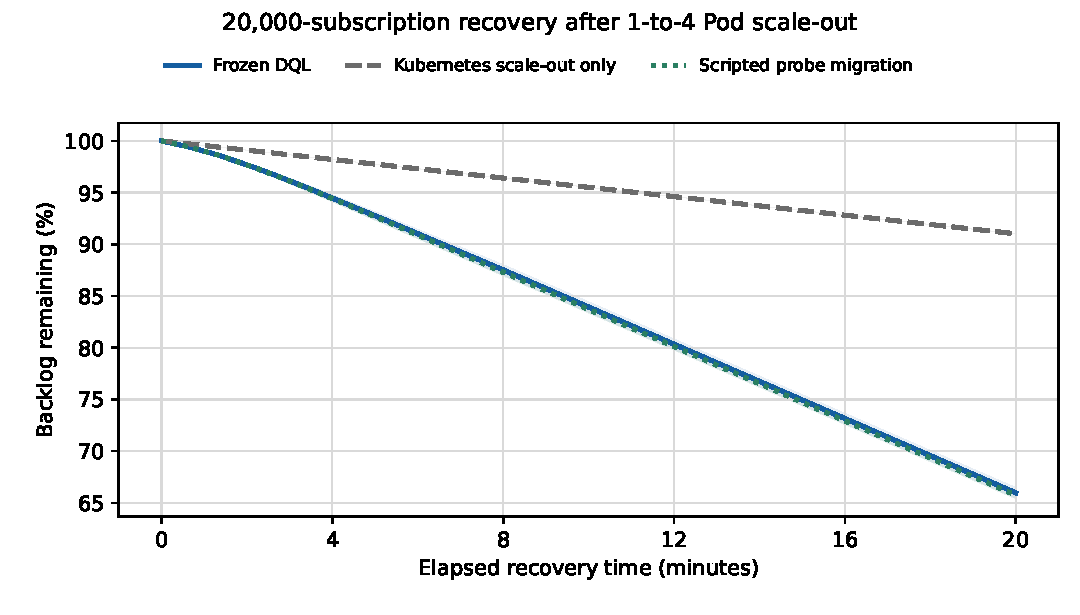
\includegraphics[width=\textwidth]{evidence/persistent-scaleout-recovery-complete/persistent_scaleout_backlog_recovery.pdf}
 \caption{Backlog recovery after adding three subscriber pods. All policies
 start with the same 775-million-event backlog. Curves are means over 20
 paired seeds; shaded bands are descriptive 95\% normal-approximation
 intervals. The area under each normalized curve defines the primary endpoint.}
 \Description{A line chart compares remaining backlog over twenty minutes.
 DQL and scripted probe migration drain substantially more backlog than
 Kubernetes scale-out with the original TCP connection placement.}
 \label{fig:scaleout-backlog-recovery}
\end{figure}

Figure~\ref{fig:scaleout-backlog-recovery} connects the endpoint to the
recovery process. The steeper DQL curve follows successful probe promotions
that place delivery work on additional pods. The nearby scripted-control curve shows that DQL reaches about the same
service capacity as guarded scripted migration. Both improve on the unchanged
placement, establishing the benefit of migration in this workload rather than
a ranking above every controller with the same actions.

Capacity-activation timelines, seed-level violin plots, and independent
ad-hoc timing controls are retained in Section~\suppref{app:scaleout-details} of
the Online Supplementary Material. Those controls do not replace the
pressure-aware guarded-greedy comparator above.

\subsection{Independent Multi-Objective Holdout}
The independent holdout compares the frozen DQL policy with the threshold-based
Heuristic and Static policies from Table~\ref{tab:policy-roles}. Full study
designs, training traces, distributions, and action-contract diagnostics are
retained in Section~\suppref{app:holdout-details}.

Table~\suppref{tab:locked-study-design} summarizes the evidence-generating runs.
In v3, three candidate networks were trained for exactly $10{,}000$
transitions under seeds 101, 211, and 307.  Candidate selection used ten fixed
validation seeds and required subscription-count rebalancing
($a^{\mathrm{reb}N}$), backlog rebalancing ($a^{\mathrm{reb}G}$), and full
connection migration ($a^{\mathrm{mig}}$) in at least $80\%$ of admissible
episodes in their intended scenarios.  Candidate 0 (seed 101) passed this gate
and was frozen before the holdout seed bank was read.

The independent v3 holdout contains ten previously unused seeds for each of
four scenarios and 500 decision intervals per episode.  The connection-count
skew scenario uses 1,000 subscriptions; the tiered-backlog scenario uses 1,200
subscriptions; and the client-slowdown and pod-pressure-skew scenarios each use
1,600 subscriptions.  Every scenario has four modeled pods, four initial
persistent connections, and a maximum of six connections.  The tiered-backlog
scenario assigns $25\%$ of its queues to each initial backlog level
$100{,}000$, $50{,}000$, $5{,}000$, and zero.  The client-slowdown scenario
reduces acknowledgement capacity to $35\%$ of its nominal value between
intervals 125 and 375.  The other two scenarios isolate initial
subscription-count skew and the placement of three of four connections on one
pod, respectively.

For policy $\pi$, paired episode $j$, and metric $v$, let
$Y_{\pi,j,v}$ denote the episode mean.  We define a direction-adjusted paired
difference
\begin{equation}
  D_{j,v}=d_v\left(Y_{\mathrm{DQL},j,v}
  -Y_{\mathrm{base},j,v}\right),
  \qquad
  d_v=\begin{cases}
  +1,&\text{higher is better},\\
  -1,&\text{lower is better}.
  \end{cases}
  \label{eq:direction-adjusted-effect}
\end{equation}
Thus, a positive $D_{j,v}$ always favors DQL.  The relative benefit reported
below is
\begin{equation}
  \mathrm{RB}_v=100\,
  \frac{\overline{D}_v}{\left|\overline{Y}_{\mathrm{base},v}\right|}.
  \label{eq:relative-benefit}
\end{equation}
Overbars in these two equations denote means across paired episodes.
The metric index $v$ is distinct from the client-population size $m$.
We resample the 40 paired differences $10{,}000$ times to obtain percentile
$95\%$ confidence intervals.  Two-sided paired sign-flip tests are exact for
the scenario-level sets of ten pairs and use $100{,}000$ Monte Carlo sign
vectors for the pooled set of 40 pairs.  Pooled $p$-values are adjusted by the
Holm procedure across the complete family of 18 metric-by-baseline tests.  The
scenario box plots in Figure~\suppref{fig:v3-scenario-reward} describe quartiles
and individual episode outcomes; the paired randomization tests
provide the statistical comparison.

We evaluate DQL as a sequential controller through return, operational
outcomes, paired effect sizes, and action coverage. Classifier accuracy and
ROC--AUC apply to labelled prediction tasks. Applying them here would mainly
measure agreement with a heuristic that supplied the correct-action labels,
rather than the controller's operating performance.

Across all 40 paired episodes, frozen DQL improves mean reward over the
heuristic from $-0.1609$ to $-0.1291$.  The mean paired difference is $0.0318$
(bootstrap 95\% CI $[0.0191,0.0455]$), equivalent to a $19.8\%$ relative
benefit under Eq.~\eqref{eq:relative-benefit}; the paired standardized effect is
$d_z=0.729$, and the Holm-adjusted sign-flip $p$-value is below $0.001$.
Table~\ref{tab:v3-paired-effects} and Figure~\suppref{fig:v3-paired-benefit} show
that this overall gain comes with tradeoffs.

\begin{table}[!htbp]
  \caption{Frozen DQL versus the heuristic on the independent v3 holdout.
  Positive benefit favors DQL.  CIs are paired-bootstrap intervals transformed
  by Eq.~\eqref{eq:relative-benefit}; $p_H$ is Holm-adjusted over 18 pooled
  metric-by-baseline tests.}
  \Description{Table listing DQL and heuristic means, direction-adjusted
  relative benefits with 95 percent confidence intervals, and Holm-adjusted
  paired sign-flip p-values for nine operational metrics.}
  \label{tab:v3-paired-effects}
  \centering
  \small
  \begin{tabular}{lrrrr}
    \toprule
    Metric & DQL & Heuristic & Benefit [95\% CI] (\%) & $p_H$ \\
    \midrule
    Mean reward & $-0.1291$ & $-0.1609$ & $19.8\ [11.9,28.3]$ & $<.001$ \\
    Backlog ratio & $0.1749$ & $0.2002$ & $12.7\ [-1.2,27.1]$ & $.095$ \\
    Conn.-subscription variance & $574.7$ & $5768.7$ & $90.0\ [61.0,120.8]$ & $<.001$ \\
    Conn.-backlog variance & $2.280\!\times\!10^{13}$ & $1.568\!\times\!10^{13}$ & $-45.4\ [-72.5,-22.6]$ & $.022$ \\
    Subscription imbalance & $0.0898$ & $0.4343$ & $79.3\ [59.1,99.5]$ & $<.001$ \\
    Backlog imbalance & $0.2194$ & $0.1638$ & $-34.0\ [-56.4,-13.6]$ & $.022$ \\
    Combined conn. imbalance & $0.1546$ & $0.2991$ & $48.3\ [33.8,63.8]$ & $<.001$ \\
    Pod pressure & $0.1878$ & $0.2051$ & $8.4\ [3.6,13.6]$ & $.022$ \\
    Throughput ratio & $0.2840$ & $0.2973$ & $-4.5\ [-7.1,-2.2]$ & $.022$ \\
    \bottomrule
  \end{tabular}
\end{table}

The largest benefit is a $90.0\%$ reduction in connection-level subscription
variance, consistent with the design objective of moving subscriptions away
from overloaded persistent connections.  Subscription imbalance falls by
$79.3\%$, combined connection imbalance by $48.3\%$, and mean pod pressure by
$8.4\%$.  Mean backlog ratio is $12.7\%$ lower, but its interval crosses zero
and the adjusted test is not significant ($p_H=.095$).  Conversely, DQL has
$45.4\%$ higher connection-backlog variance, $34.0\%$ higher normalized backlog
imbalance, and $4.5\%$ lower throughput than the heuristic.  The scalar reward
still favors DQL because its configured penalties place substantial weight on
subscription pressure and combined imbalance. The holdout therefore identifies
a multi-objective advantage for DQL and a queue-drainage advantage for the
heuristic.

\subsection{Adverse-Probe Ablation}
The separate 30-seed, 1,200-subscription ablation compares the same frozen DQL
policy with and without one forced promotion to the highest-pressure probe
Pod. Guarded DQL reduces normalized backlog AUC from 0.68938 to 0.66046:
a paired difference of $-0.028918$ (95\% CI $[-0.039444,-0.019073]$), or 4.19\%.
The guarded heuristic retains the lower AUC of 0.59104. This isolates the
benefit of guarding promotion, not universal superiority of learned selection.
The complete five-policy comparison, methods, and separate five-seed
20,000-subscription confirmation are retained in
Section~\suppref{sec:adverse-probe-ablation}.
\paragraph{Reviewer artifact access.}
The accompanying supplementary archive, \texttt{reviewer-evidence.zip},
contains episode-level simulator CSVs, declared protocols, original aggregate
analyses, the frozen 21--32--6 checkpoint, and identifier-free live summaries.
Its README gives the file map and exact offline commands. A Python 3.9+
standard-library script verifies the checksum manifest, checks paired cohort
coverage, recomputes policy means and selected effect sizes, and reconciles
the loaded trial's reported subscription and ACK totals. A separate inference
option evaluates the saved network without transport access or model updates.
The archive supports reanalysis and checkpoint inspection; it does not expose
corporate credentials, raw event payloads, private endpoint identifiers, or
the proprietary service source. It is not a complete independent deployment
rerun. Provenance records distinguish unchanged measurements from redacted
local-path metadata.

The public research repository is available at
\url{https://github.com/manish94u/rebalancePersistance}.
It provides the manuscript sources, standalone simulator, redacted evidence,
frozen checkpoint, and step-by-step replication instructions.

\section{Stability Controls and Policy Validation}

Because the controller operates with partial and periodically refreshed
statistics, stability is enforced at two levels.  During learning, replay,
target-network synchronization, bounded rewards, and epsilon decay limit the
rate at which value estimates change.  During execution, feasibility masks,
minimum-improvement thresholds, cooldowns, and the receipt-gated handoff protocol
prevent a high Q-value from bypassing required operating rules. These controls
bound the available transitions. Their role is operational stability, distinct
from a proof of learned-policy convergence.

Classical tabular Q-learning guarantees assume a stationary, fully observable
Markov decision process and sufficient visitation of every state-action pair.
The client instead receives delayed partial observations in an environment
whose queue arrivals, acknowledgement capacity, and competing clients can
change. Policy quality is therefore evaluated under the stated workloads,
without a global-optimality guarantee. The finite v3 traces describe training
behavior rather than Bellman-loss convergence. The v4--v6 results distinguish
training completion from action coverage. The validation protocol uses
action-coverage, fault-safety, churn, and performance gates to assess each
frozen policy.

RL evaluation also separates adaptation from regression. Biagiola and Tonella
test how RL systems adapt to changed environments while retaining prior
capabilities \cite{Biagiola2022Plasticity}. Patterson et al. discuss performance
variation, baseline construction, hyperparameter selection, and experimenter
bias in empirical RL \cite{Patterson2024EmpiricalDesign}. These concerns motivate
reporting the training, frozen-policy comparison, and live handoff evidence
separately. A successful handoff and a higher comparative reward answer
different evaluation questions.

\section{Discussion}

The main systems finding is that subscriber capacity and client access to that
capacity are separate. Adding Pods supplies service capacity; moving existing
subscription-bearing connections makes it reachable by persistent clients.
The guarded-greedy and DQL policies both achieve this in the scale-out model.
Their nearby throughput results support the shared mechanism rather than
requiring a claim that learning beats a strong greedy rule in every workload.

Policy choice depends on the operational objective. Greedy control gives a
direct, inspectable response to measured pressure. DQL can account for delayed
costs and several competing objectives. A subscription move changes future
backlog distribution; migration trades immediate handoff cost for later
capacity. Both selectors operate above the same bounded, checked actions.

The action-contract studies provide a further design lesson: a useful
executor and a policy that reliably selects it are separate requirements.
The cap-restoring scale-up preflight improved reward and maximum subscription
count, but the expanded learner study did not pass every coverage gate.
Appendix~\suppref{app:action-diagnostics} retains these results. They explain why
the live checkpoint uses a compatible, restricted rebalancing profile.

\section{Conclusion}

We presented a probe-guided, client-side framework for rebalancing
persistent subscription connections without requiring cluster-wide client
visibility.  The mechanism combines per-subscription queues, active-connection
telemetry, and a load-balancer-assigned probe. Greedy rules or DQL select
bounded actions, and a shared executor carries out receipt-gated handoff.
The technical contribution is the link between partial observations,
endpoint-preserving probe promotion, and selective subscription reassociation.

The primary experiment demonstrates recovery after a one-to-four pod capacity
increase with 20,000 subscriptions and 775 million queued events. Guarded-greedy
migration and frozen DQL deliver 221,260 and 219,762 events/s, respectively,
compared with 58,000 events/s for unchanged placement. Frozen DQL
uses all four pods, delivers 3.79 times the mean throughput, and leaves 27.52\%
less backlog after 20 minutes than retaining the ten original connection
assignments. Its 12.30\% reduction in backlog area satisfies the registered
paired statistical criterion. The adverse-probe ablation complements this
result: evaluating the candidate before promotion reduces backlog area by
4.19\% relative to forcing one harmful migration.
The Oracle Cloud experiments establish live handoff execution, subscription
retention, and observed delivery behavior. The comparative throughput and
backlog-recovery gains are simulator measurements under the stated service
assumptions. These results support two evaluated policy options above the same
probe-guided handoff mechanism.

\FloatBarrier
\bibliographystyle{ACM-Reference-Format}
\bibliography{example}
\end{document}
